\documentclass{article}

\usepackage[version=3]{mhchem} % Package for chemical equation typesetting
\usepackage{siunitx} % Provides the \SI{}{} and \si{} command for typesetting SI units
\usepackage{graphicx} % Required for the inclusion of images
\usepackage{natbib} % Required to change bibliography style to APA
\usepackage{amsmath} % Required for some math elements 
\usepackage{graphicx}

\setlength\parindent{0pt} % Removes all indentation from paragraphs

\begin{document}
\section{Road Construction}
This module is tend to find the best road building method. The strategies we have tried include global ones and local ones, which will be explained in each subsection.
\subsection{Shortest path approach}
The most simple but also efficient way to build road is choose the shortest one from existing road an edges to the picked best build place. The implementation of shortest path is simple. it also observe the idea to build road as less as possible, as the road cells make no profits. The shortest path cause closed vacant areas sometimes, but in most of the cases, the closed area will be largely filled by later coming buildings. We also have tried to build the roads cling to existing buildings, but it got lower scores.
\subsection{Road pre-building}
Because the online build road algorithm can disturb the building order, we also have tried several pre-build approaches. Before the request coming, we pre-build some road in a tree-like(fractal) fashion. The idea behind is to let the road touch larger areas efficiently. But this approach also lower the score gained. After several experiments, we got the sense that pre-build is not a good idea in this game, as it add more constraints to the later planning.
Figure \ref{fig: prebuildRoad} demonstrate the tree-like pre-build approach.

\begin{figure}
\center
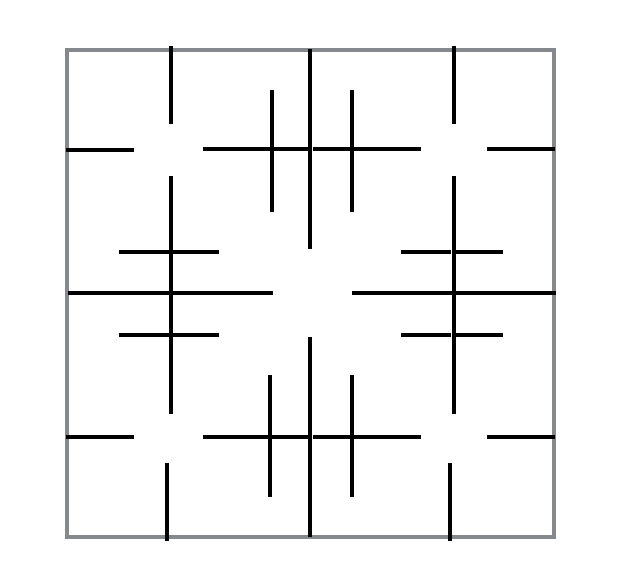
\includegraphics[scale=0.5]{prebuildRoad.png}
\caption{roads grow in fractal manner}
\label{fig: prebuildRoad}
\end{figure}

\subsection{close to the buildings}
After dozens of experiments, we finally choose the simple but efficient shortest path strategy. But add an second key which is measure the perimeter of the road. The perimeter is defined in the same way with the building perimeter we mentioned in the last section. Then, our submitted version choose the road with maximum perimeter among those has the shortest length. This feature makes little difference in the performance, not considerably higher but also not considerably lower.
\end{document}